% Options for packages loaded elsewhere
\PassOptionsToPackage{unicode}{hyperref}
\PassOptionsToPackage{hyphens}{url}
%
\documentclass[
]{article}
\usepackage{lmodern}
\usepackage{amssymb,amsmath}
\usepackage{ifxetex,ifluatex}
\ifnum 0\ifxetex 1\fi\ifluatex 1\fi=0 % if pdftex
  \usepackage[T1]{fontenc}
  \usepackage[utf8]{inputenc}
  \usepackage{textcomp} % provide euro and other symbols
\else % if luatex or xetex
  \usepackage{unicode-math}
  \defaultfontfeatures{Scale=MatchLowercase}
  \defaultfontfeatures[\rmfamily]{Ligatures=TeX,Scale=1}
\fi
% Use upquote if available, for straight quotes in verbatim environments
\IfFileExists{upquote.sty}{\usepackage{upquote}}{}
\IfFileExists{microtype.sty}{% use microtype if available
  \usepackage[]{microtype}
  \UseMicrotypeSet[protrusion]{basicmath} % disable protrusion for tt fonts
}{}
\makeatletter
\@ifundefined{KOMAClassName}{% if non-KOMA class
  \IfFileExists{parskip.sty}{%
    \usepackage{parskip}
  }{% else
    \setlength{\parindent}{0pt}
    \setlength{\parskip}{6pt plus 2pt minus 1pt}}
}{% if KOMA class
  \KOMAoptions{parskip=half}}
\makeatother
\usepackage{xcolor}
\IfFileExists{xurl.sty}{\usepackage{xurl}}{} % add URL line breaks if available
\IfFileExists{bookmark.sty}{\usepackage{bookmark}}{\usepackage{hyperref}}
\hypersetup{
  hidelinks,
  pdfcreator={LaTeX via pandoc}}
\urlstyle{same} % disable monospaced font for URLs
\usepackage{graphicx}
\makeatletter
\def\maxwidth{\ifdim\Gin@nat@width>\linewidth\linewidth\else\Gin@nat@width\fi}
\def\maxheight{\ifdim\Gin@nat@height>\textheight\textheight\else\Gin@nat@height\fi}
\makeatother
% Scale images if necessary, so that they will not overflow the page
% margins by default, and it is still possible to overwrite the defaults
% using explicit options in \includegraphics[width, height, ...]{}
\setkeys{Gin}{width=\maxwidth,height=\maxheight,keepaspectratio}
% Set default figure placement to htbp
\makeatletter
\def\fps@figure{htbp}
\makeatother
\setlength{\emergencystretch}{3em} % prevent overfull lines
\providecommand{\tightlist}{%
  \setlength{\itemsep}{0pt}\setlength{\parskip}{0pt}}
\setcounter{secnumdepth}{-\maxdimen} % remove section numbering

\author{}
\date{}

\begin{document}

\hypertarget{header-n0}{%
\section{UML Use Case Diagram Editor based on GLSP}\label{header-n0}}

Using the UML Use Case Diagram Editor is quite simple. After creating a
new file you can add any element to the canvas by selecting the
corresponding tool from the tool pallet.

\hypertarget{header-n186}{%
\subsection{Creating a new Use Case Diagram}\label{header-n186}}

A new diagram can be created via:

\begin{itemize}
\item
  via menu entry
  \texttt{File\ -\textgreater{}\ New\ UML\ Class\ Diagram}
\item
  via explorer context menu entry \texttt{New\ UML\ Class\ Diagram}
\item
  via command palette \texttt{File:\ New\ UML\ Class\ Diagram}
\end{itemize}

Afterwards the diagram needs to be named:

\begin{figure}
\centering
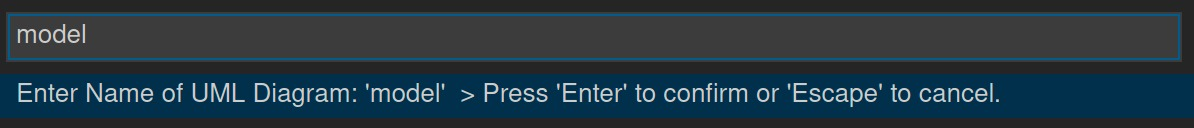
\includegraphics{C:/Users/Lukas/Documents/01_Studium/Master/03_Sommer2021/AME/use_case_diagram/figures_for_readme/ScreenShotNaming.jpeg}
\caption{}
\end{figure}

and the type of the diagram needs to be specified. In the case of Use
Case diagrams \texttt{usecase} needs to be entered

\begin{figure}
\centering
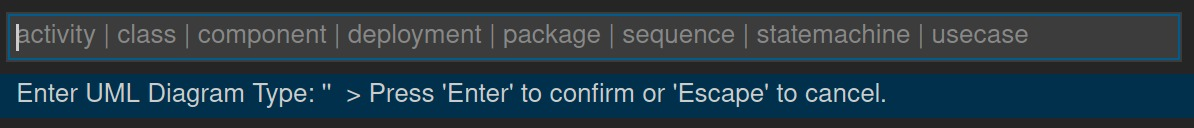
\includegraphics{C:/Users/Lukas/Documents/01_Studium/Master/03_Sommer2021/AME/use_case_diagram/figures_for_readme/ScreenShotTypeSelection.jpeg}
\caption{}
\end{figure}

Afterwards an empty modelling canvas will be displayed.

\begin{figure}
\centering
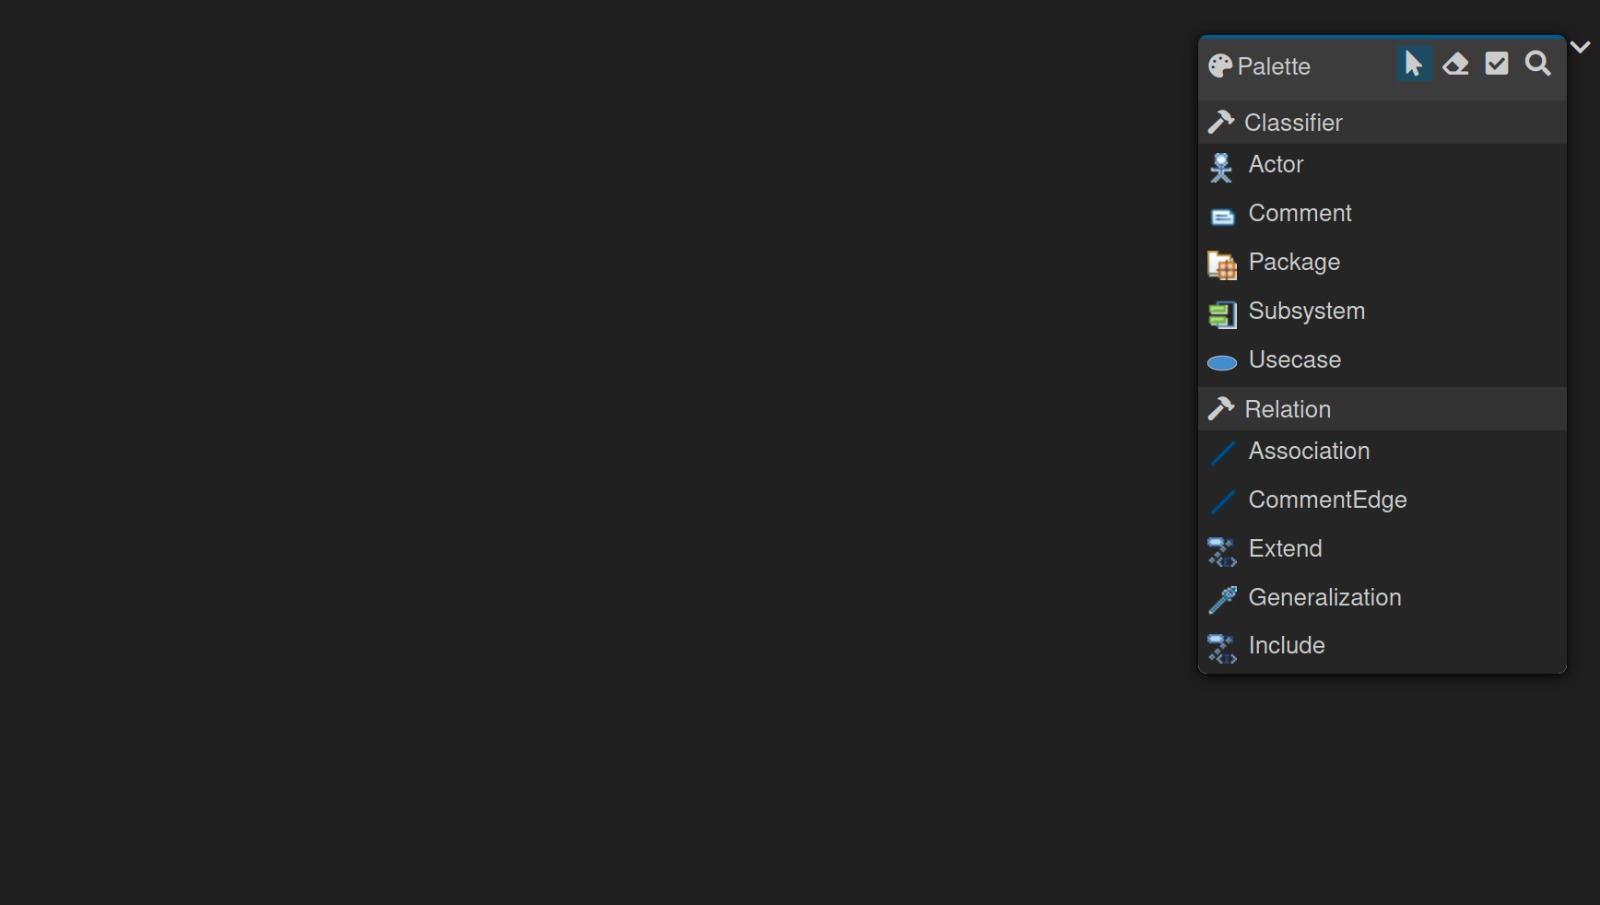
\includegraphics{C:/Users/Lukas/Documents/01_Studium/Master/03_Sommer2021/AME/use_case_diagram/figures_for_readme/ScreenShotCanvas.jpeg}
\caption{}
\end{figure}

\hypertarget{header-n216}{%
\subsection{Starting to model}\label{header-n216}}

To build your first model just click on the tool in the pallet for the
element you want to add and click on the canvas.

For creating edges between to elements, first select a relation tool,
second select the source element and last select the target element. The
cursor will change depending on whether creating a relationship between
the two elements is allowed.

Comments can be either added to the canvas or directly to the element to
be annotated, depending on whether it is clicked on the canvas or on the
element to be annotated. Comments can be added to classifiers but also
to extend edges (note there is an existing bug regarding the rendering
of the edge between the comment and the extend edge)

Subsystems and Packages have child compartments to which element can be
added by selecting them and clicking on the parent (Subsystem or
Package). Subsystems can only take use cases as children, packages can
take any classifier.

\end{document}
